
\documentclass[a4paper,12pt]{article}
\usepackage{../acn-scientific}
\usepackage{../acn-particlestyle}
\usetikzlibrary{decorations.pathreplacing,
  decorations.markings,
  decorations.pathmorphing}

\setcounter{secnumdepth}{0}

%\addtolength{\voffset}{-2cm}
%\addtolength{\textheight}{4cm}

%\title{AQA Unit PHYA1\\Particles, Quantum Phenomena and Electricity}
\title{AQA Unit PHYA1\\Particles and Radiation}
\author{Mr \textsc{A.C. Norman}\\
\textsc{Bishop Heber High School}
\\ \texttt{anorman@bishopheber.cheshire.sch.uk}}
\date{Autumn Term, 2012}

\begin{document}
\begin{titlepage}
\maketitle

\thispagestyle{empty}
\enlargethispage{4cm}
	
\noindent\includegraphics[width=\textwidth]{img/large_hadron_collider.png} 

\begin{flushright}
\texttt{http://xkcd.com/401/}
\end{flushright}
\end{titlepage}
\newpage

\thispagestyle{empty}
\addtocounter{page}{-1}

\begin{center}
\fbox{
\begin{minipage}{0.7\textwidth}
\vspace*{1em}
\begin{center}
\includegraphics[width=0.3\textwidth]{../by-nc-sa.png}
\end{center}

This work is licensed under a Creative Commons
Attribution-NonCommercial-ShareAlike License.

{\footnotesize\texttt{http://creativecommons.org/licenses/by-nc-sa/3.0/}}\\

Non-commercial uses are thus permitted without any
further permission from the copyright owner.\\

%Permissions beyond the scope of this license are
%administered by the author. Information on how
%to request permission may be found at:
%http://www.randomhouse.com/about/
%permissions.html
\end{minipage}
}
\end{center}

%\tableofcontents
\clearpage
%\part{Waves}

%CONTENT:


\section{Constituents of the atom}

The atom comprises a tiny ($\approx \SI{e-14}{m}$) nucleus, containing protons and neutrons, around which are electrons in atomic orbitals (of radius $\approx \SI{e-10}{m}$).

\begin{table}[ht]
  \centering
  \fontfamily{ppl}\small\selectfont
  \begin{tabular}{lcccc}
    \toprule
    Name & Location & Charge / C & Relative mass & Actual mass / kg\\
    \midrule
    Proton & nucleus & +\num{1.6e-19} & 1 & \num{1.67e-27}\\
    Neutron & nucleus & 0 & 1 & \num{1.67e-27}\\
    Electron & orbitals & $-$\num{1.6e-19} & $1/1833$ & \num{9.11e-31}\\
    \bottomrule
  \end{tabular}
  \caption{The particles which make up matter and their properties.}
\end{table}

An atom is written as

\begin{center}
{\huge \isotope[{\it A}][{\it Z}]{X}}
\end{center}

where \begin{minipage}[t]{12cm}$A$ is the nucleon number (the number of protons and neutrons),\\
$Z$ is the proton number, and\\
X is the element symbol.\end{minipage}

\subsection{Proton number, $Z$}

Also called the atomic number.  This defines the element, and therefore dictates its properties.  In an atom, the number of electrons will equal the proton number; in an ion, there will be fewer or more electrons than $Z$.

\subsection{Nucleon number, $A$}

Also called the mass number.  This is the total number of nucleons (i.e.\ protons + neutrons) in the nucleus.

The number of neutrons is therefore $A-Z$.  All nuclei, except for one isotope of hydrogen, contain neutrons.\footnote{In general, for lower $Z$ elements, there are roughly the same numbers of protons and neutrons, but the number of neutrons increases more rapidly as large nuclei are made.}  The neutrons hold together the protons, which electrostatically repel each other.

The number of neutrons have no effect on the chemical properties of the element, but may make it more or less stable and therefore determine whether an element is radioactive.

\subsection{Isotopes}

Isotopes are nuclides with the same proton number, but different nucleon numbers (i.e.\ same number of protons, but different numbers of neutrons).

Many elements exist in several stable isotopes, and they are not given separate names, except for:
\begin{itemize}
\item \isotope[1][1]{H} is hydrogen.
\item \isotope[2][1]{H} is deuterium.
\item \isotope[3][1]{H} is tritium.
\end{itemize}

%nuclearstability.pdf
%nuclearstabilityblanks.pdf
\section{Nuclear stability}

Within a nucleus, which normally has a diameter of about \SI{e-14}{m}, a large attraction force is needed to overcome the coulomb repulsion of the very closely packed protons.\footnote{The magnitude of this force is of the order \SI{e4}{N}.}

Experimental investigations of nuclear material show that it is very dense, and the density is independent of the nucleon number.  This implies that the force between nucleons is a short range force, only extending to the adjacent nucleons (if it extended further a density increase with $A$ would be expected, as more and more nucleons pulled tighter and tighter on each other!)

The nuclear force---called the strong force---is very complex and it is not possible to deduce its form precisely.  However, we can note that
\begin{itemize}
\item it is essential to keep the nucleus stable and bound together (balancing the effect of proton--proton electrostatic repulsion)
\item it is about \num{e8} times stronger than interatomic forces
\item it is charge independent, i.e.\  at any given separation the strong force between two neutrons is the same as that between two protons or between a proton and neutron
\item it is attractive down to about \SI{3}{fm}=\SI{3e-15}{m}
\item it has to be repulsive at very short range ($<0.5$~fm) otherwise there would be a tendency for the nucleus to collapse in on itself
\end{itemize}

\section{Radioactivity}

Radioactivity is the spontaneous disintegration of the nucleus of an atom, from which may be emitted some or all of the following 
\begin{itemize}
\item $\alpha$ alpha particles,
\item $\beta$ beta particles,
\item $\gamma$ gamma rays.
\end{itemize}

The process allows an unstable nucleus to become more stable, and its rate is not affected by chemical combinations or changes in physical environment.  Natural sources of background radiation (which must be taken into account when taking experimental radioactivity measurements) include cosmic rays, rocks (especially granite) and some luminous paints.

\subsection{$\alpha$ decay}
An $\alpha$ particle is identical to a helium nucleus, consisting of 2 protons and 2 neutrons.

When an element disintegrates by the emission of an $\alpha$ particle it turns into an element with chemical properties similar to those of an element two places earlier in the periodic table $(A,Z)\rightarrow(A-4,Z-2)$.

e.g.\ Radium  decays via $\alpha$ emission to form radon (Rn):
\[\isotope[226][88]{Ra}\longrightarrow\isotope[222][86]{Rn}+\isotope[4][2]{\alpha}.\]

\subsection{$\beta$ decay}
A $\beta$ particle is an electron. During $\beta$ decay a neutron changes into a proton.  When an element disintegrates by emission of a $\beta$ particle it turns into an element with chemical properties similar to an element one place later in the periodic table $(A,Z)\rightarrow(A,Z+1)$. 

e.g.\  Sodium-24 (also known as radiosodium) decays via $\beta$ emission to magnesium-24:
\[\isotope[24][11]{Na}\longrightarrow\isotope[24][12]{Mg}+\isotope[0][-1]{\beta}.\]

\subsection{$\gamma$ radiation}

Frequently, spare energy released during a radioactive disintegration is emitted as very penetrating and harmful $\gamma$ radiation (very short wavelength electromagnetic radiation).  Though the nucleus loses energy by $\gamma$ emission, the structure of the nucleus $(A,Z)$ does not change.

%fourforces.pdf
%fourforcesblanks.pdf
\section{Particles and their antiparticles}

Every particle that exists has an antiparticle.  Antiparticles do not exist as constituents of ordinary matter, but are easily created in particle accelerators, and are produced in radioactive decay and cosmic rays.

For every particle:
\begin{itemize}
\item its antiparticle has the same mass
\item its antiparticle has equal but opposite charge (as well as other associated numbers)
\item an unstable particle has the same half-life as its antiparticle
\end{itemize}

\subsection{Stable particles}

The following particles are the only particles which are stable:\\

\begin{table}[ht]
  \centering
  \fontfamily{ppl}\selectfont
  \begin{tabular}{lcccc}
    \toprule
    Name & Symbol & Charge ($Q$) / $e$ & Rest mass / kg & Rest energy / MeV\\
    \midrule
    electron & \Pelectron & $-1$ & 9.1\e{-31} & 0.511\\
    positron & \Ppositron & $+1$ & 9.1\e{-31} & 0.511\\
    proton & \Pproton & $+1$ & 1.6\e{-27} & 938\\
    antiproton & \APproton & $-1$ & 1.6\e{-27} & 938\\
    neutrino & \Pnu & 0 & $\sim 10^{-37}??$ & $<\num{18.2e-6}$\\
    antineutrino & \APnu & 0 & $\sim 10^{-37}??$ & $<\num{18.2e-6}$\\
    \bottomrule
  \end{tabular}
%  \caption{The particles which make up matter and thei}
\end{table}

\paragraph{Notes}\begin{enumerate}
\item The electron volt (eV) is a unit of {\bf energy}.\footnote{The electron volt is the amount of energy gained by an electron when it is accelerated through a potential difference of 1 volt.}  In atomic and nuclear physics, the joule is too large a unit for convenience.
\[\SI{1}{eV}=\SI{1.6e-19}{J}\text{ and }\SI{1}{MeV}=\SI{e6}{eV}.\]
\item The antiparticles are stable in isolation: in practice, they would likely encounter a particle and annihilate if they came into contact with normal matter.
\item There are three kinds of neutrino, and therefore three antineutrinos.\footnote{In fact, neutrinos are constantly shifting between these three flavours of neutrino -- this is how physicists know they have mass!}
\item Some particles are identical to their anti-particle, e.g.\ the photon, and the \Ppizero (pi-meson).
\item In general, particle symbols are made into their antiparticle by the `bar' above the symbol.
\end{enumerate}

\subsection{Neutrinos}
The neutrino was predicted to exist in 1930, and was postulated due to the range of energies of beta particles in radioactive beta decay.

Neutrinos are the most common particles in the universe, outnumbering the number of protons by about a billion to one.  They are emitted in nuclear reactions such as those that occur inside the sun.

They are very difficult to detect, even though 6\e{10} pass through every square centimetre of the earth every second.  They interact very weakly, and this is why their mass was not discovered until recently, and is an area of ongoing research.

\subsection{Photons}

Light, and all of the electromagnetic spectrum, can be described as a wave, and this adequately explains effects such as diffraction and reflexion.  However, physicists found that some phenomena, such as the photoelectric effect\footnote{This is discussed in more detail in `quantum phenomena'.  Briefly, it is the emission of electrons from the surface of a metal.  It is noted that (i) there is a minimum frequency of light to cause emission (the electrons need a minimum energy to escape) and (ii) the kinetic energy of the electrons emitted increases as the frequency of the light increases (photons have more energy to give to the electrons).} and the black body radiation spectrum\footnote{You don't have to know about this at A-level.}, could not be described in this way.

In 1900, Max Planck came up with a suggestion that objects which emit electromagnetic radiation do so in discrete amounts.  He said that the energy was proportional to the frequency of the radiation, i.e.
\[E\propto f,\mathrm{~or}\]
\[E=hf,\]
where $h$ is the Planck constant, \SI{6.64e-34}{J.s}.

The individual packets, or quanta, of electromagnetic radiation are called photons.  Photons are indivisible, and when they collide with e.g.\ an electron, all or none of the energy is given to the electron.

\paragraph{Examples}

\begin{fullwidth}
\begin{enumerate}
\item Calculate the photon energy of
\begin{enumerate}
\item a gamma ray of frequency 2\e{22}~Hz\\
$E=hf=6.64\e{-34}~\mathrm{J~s~}\times 2\e{22}~\mathrm{s}^{-1}=1.33\e{-11}$~J.
\item red light of wavelength 7.8\e{-7}~m\\
$E=hf$, as $c=f\lambda$ (where $c=3\e{8}$~m~s$^{-1}$)\\
$E=\dfrac{hc}{\lambda}=\dfrac{6.64\e{-34}~\mathrm{J~s~}\times 3\e{8}~\mathrm{m~s}^{-1}}{7.8\e{-7}~\mathrm{m}}=2.55\e{-19}$~J.
\end{enumerate}
\item A sodium light emits yellow light of frequency 5.1\e{14}~Hz.  If it is a 30~W lamp, how many photons are emitted per second?\\
$30~\mathrm{W}=30$~J~s$^{-1}.$\\
$P=\dfrac{E}{t}=\mathrm{photon~number~per~unit~time}\times hf,$\\
$\mathrm{photon~number~per~unit~time}=\dfrac{P}{hf}=\dfrac{30~\mathrm{J}~\mathrm{s}^{-1}}{6.64\e{-34}~\mathrm{J~s~}\times 5.1\e{14}~\mathrm{Hz}}=8.9\e{19}~\mathrm{s}^{-1}.$
\end{enumerate}
\end{fullwidth}

%antiphotons.pdf
%antiphotonsblanks.pdf
%annihilationpairproduction.pdf
%annihilationpairproductionblanks.pdf

Elementary particles are affected by only four fundamental forces (or `interactions').  Gravity and the electromagnetic interaction are already familiar forces from our everyday experience, and in addition there are two nuclear forces, the strong interaction and the weak interaction.

\begin{table}
  \centering
  \fontfamily{ppl}\small\selectfont
  \begin{tabular}{lcc}
    \toprule
    Interaction & Range / m & Relative strength\\
    \midrule
    Strong & $\sim 10^{-15}$ & 1\\
    Electromagnetism & $\infty$ & $10^{-2}$\\
    Weak & $\sim 10^{-18}$ & $\sim 10^{-7}$\\
    Gravity & $\infty$ & $\sim 10^{-39}$\\
    \bottomrule
  \end{tabular}
  \caption{Summary of all four fundamental interactions.}
\end{table}

\subsection{Gravity}
Gravity affects all particles which have mass.  It has an infinite range and is purely attractive.  It governs the structure of stars, galaxies \&{}c.\ and its exact strength will determine the fate of the universe.

\subsection{Electromagnetism}
This interaction affects all particles with charge.  It is much stronger than gravity and also of infinite range, but it tends to cancel in bulk matter as this normally comprises nearly exactly equal numbers of positively and negatively charged particles.

\subsection{Strong}

The strong interaction is only felt by hadrons, which are all made from quarks.  The strong interaction is short range, and only affects nearest neighbours in the nucleus, as its range is the same as the diameter of a nucleon.  The strong interaction is always attractive, and charge independent (the same for n--p, p--p and n--n).

\begin{figure}
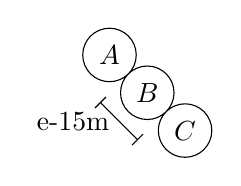
\begin{tikzpicture}[scale=1.2]
\draw (-0.4,0.4) node {$A$} circle (0.283) (0,0) node {$B$} circle (0.283) (0.4,-0.4) node {$C$} circle (0.283);
\draw[|-|] (-0.3,-0.3) node[anchor=east] {\SI{e-15}{m}} ++(-0.2,0.2)--++(0.4,-0.4);
\end{tikzpicture}
\caption{The strong interaction only affects nearest neighbours, i.e.\ $A$ and $B$ are attracted by the strong interaction, as are $B$ and $C$, but $A$ and $C$ are not.}
\end{figure}

\subsection{Weak}

When a neutron decays into a proton and an electron, an antineutrino is formed.  This is uncharged and does not feel the strong interaction, so another short range interaction must be involved.  The weak interaction affects both hadrons and leptons, and is usually associated with decays of various particles.  Weak decays generally take place much more slowly than strong decays (the stronger the interaction, the quicker the decay).

When \emph{strange} particles decay, they do so by the weak interaction, and strangeness is not conserved.

\subsection{Modern explanation of the four interactions}

It was previously thought that a particle creates a field which exists throughout all space, and this field affects any particles in the field, causing them to experience forces.  The modern view, however, is that two particles exert a force on one another due to the transfer of a virtual particle, which carries the interaction (this is known as second quantization).  These particles are called exchange particles, and are gauge bosons.

The amount of energy `borrowed' to create the mass/energy of the exchange particle\footnote{The energy to create these particles is `borrowed' according to the Heisenberg uncertainty principle, which allows energy $\Delta E$ to be created for a time $\Delta t$, so long as
\[\Delta E \times \Delta t < \hbar,\]
where $\hbar=\dfrac{h}{2\pi}=\SI{1.05e-34}{J.s}$, known as the reduced Planck constant.  Since the product of the energy and the time has to be below a certain limit, more massive exchange particles cannot exist for a long time, putting a limit on how far they may travel, and thus the range of the interaction.
} puts an upper limit on the range of the interactions produced.  This suggests:
\begin{itemize}
\item The range of electromagnetic and gravitational interactions is infinite, so the exchange particles for these interactions must be massless.
\item The range of the strong and weak are finite, so the exchange particles have mass, and the mass of the weak exchange particle is larger.
\end{itemize}

\subsection{The strong interaction}

Protons and neutrons are held together by the strong interaction (which acts on all hadrons).  As the range of the strong interaction is \SI{e-15}{m}, and assuming the exchange particle has a speed close to that of light, it must exist for \SI{e-23}{s}.  This allows the mass of the exchange particle to be calculated, and it is found that the particle is the pi-meson or pion.

\begin{figure}
\begin{tikzpicture}[scale=0.8]
\draw[style={boson}]
  (0, 0) -- node[auto] {$\pi^{0}$} (2,0) ;
    \draw[style={electron}]
   (-1, -2) -- node[left] {\Pproton} (0, 0);
  \draw[style={electron}]
  (0, 0) -- node[left] {\Pproton} (-1, 2) ;
  \draw[style={electron}]
   (3, -2)  -- node[right] {\Pneutron} (2, 0) ;
  \draw[style={electron}]
  (2, 0) -- node[right] {\Pneutron} (3, 2) ;
\end{tikzpicture}
\end{minipage}
\begin{minipage}{0.5\textwidth}
\caption{A representation of the strong interaction between a proton and a neutron.  The direction of the paths does not show the direction of the particles, only of the interaction.}
\end{figure}

\begin{marginfigure}
\begin{tikzpicture}[scale=0.5]
\draw[style={gluon}]
  (0, 0) -- node[auto] {\Pgluon} (2,0) ;
    \draw[style={electron}]
   (-1, -2) -- node[left] {\Pup}(0, 0);
  \draw[style={electron}]
  (0, 0) -- node[left]{\Pup}(-1, 2) ;
  \draw[style={electron}]
   (3, -2) --node[right] {\Pdown}  (2, 0) ;
  \draw[style={electron}]
  (2, 0) -- node[right] {\Pdown} (3, 2) ;
\draw[white](-1,0)--(3,5);%spacer
\end{tikzpicture}
\caption{At a deeper level, the quarks themselves in the hadrons are held together by the strong force, via gluons.  The pion in the interaction between the proton and the neutron can be seen to exist to carry the gluons between the hadrons.}
\end{marginfigure}

\subsection{The weak interaction}

The weak interaction is very short range which suggests the exchange particle is massive.  One of the characteristics of the weak interaction is that it is responsible for decays of particles.  The weak interaction causes a change in the quark structure of a hadron.

There are three particles which can carry the weak interaction, \PWplus, \PWminus and \PZzero, and these act on leptons and hadrons.

The most common weak interaction is beta decay.  In this, a neutron decays into a proton, and into an electron and anti-electron neutrino through the weak interaction:
\[\Pneutron\longrightarrow\Pproton+\Pelectron+\APnue.\]

\begin{figure}
\begin{tikzpicture}[scale=0.8]
\draw[style={boson}]
  (0, 0) -- node[below] {\PWminus} (2,0) ;
   \draw[->] (0.5,-0.6)--(1.5,-0.6);
    \draw[style={electron}]
   (-1, -2) -- node[left] {\Pneutron}(0, 0);
   
  \draw[style={electron}]
  (0, 0) -- node[left] {\Pproton}(-1, 2) ;
  \draw[style={electron}]
   (2, 0)  -- node[right] {\Pelectron}(1, 2) ;
  \draw[style={electron}]
  (2, 0) -- node[right] {\APnue}(3, 2) ;
\end{tikzpicture}  
\caption{The \PWminus is the carrier of this weak interaction.  It needs to be negative to conserve charge.}
\end{figure}

The weak interaction is the only interaction which acts on neutrinos (other than gravity), and this is why they are weakly interacting.

The weak interaction is responsible for the changing of a strange quark into a non-strange quark, and this is why strangeness can sometimes change in a weak decay.

\subsection{Electromagnetism}

The electromagnetic interaction is exerted between any charged particles, and is described by the theory known as \emph{quantum electrodynamics (QED)}.  As the range of the interaction is infinite, the exchange particle is massless, and is a virtual photon.

\begin{figure}
\begin{tikzpicture}[scale=0.8]
\draw[style={boson}]
  (0, 0) -- node[auto] {\Pphoton} (2,0) ;
    \draw[style={electron}]
   (-1, -2) -- node[left] {\Pelectron}(0, 0);
  \draw[style={electron}]
  (0, 0) -- node[left] {\Pelectron}(-1, 2) ;
  \draw[style={electron}]
   (3, -2)  -- node[right] {\Pelectron}(2, 0) ;
  \draw[style={electron}]
  (2, 0) -- node[right] {\Pelectron}(3, 2) ;
\end{tikzpicture}
\caption{An example of the electromagnetic interaction is this electron--electron elastic scattering event.}
\end{figure}

\subsection{Gravity}
The particle responsible for the gravitational interaction is postulated to be the graviton.  It ought to have zero mass and zero charge, but has not yet been detected.

\subsection{Unification}
It is believed that all four interactions can be theoretically united,\footnote{There has been some success already---unification of electromagnetic and weak---and it is an aim of modern physics to find a `grand unified theory' or `theory of everything' encompassing all four interactions\ldots} to show that they are all different aspects of one interaction.

%fourforcesextra.pdf
\section{Classification of particles}
All fundamental particles fall into one of three families: the leptons, the quarks, and the gauge bosons.

\subsection{Leptons}

There are twelve different leptons, which do not experience the strong interaction (and uncharged leptons do not feel the electromagnetic interaction either).  They are the electron, the muon and the tau, each has an associated neutrino, and they all have antiparticles.  The standard model, a collection of related gauge theories currently used in particle physics, suggests that these are the only leptons which exist.  The electron and positron are stable.

The muon (\Pmuon) was discovered in cosmic rays in 1937, and has the same charge as the electron, but is 207 times heavier.  The neutrino which accompanies its reactions was found to be different from the neutrino in electron reactions in 1962.

The tau (\Ptauon) was discovered in 1978, and is also the same charge as the electron, but is around 3500 times more massive.  The neutrino that accompanies the tau was only discovered in 2000 (leaving the Higgs boson as the last particle in the standard model to be observed in 2012), though both particles' existence was assumed in the standard model long before this.

Both the muon and the tau decay into electrons.

\begin{table}
  \centering
  \fontfamily{ppl}\small\selectfont
  \begin{tabular}{lccccc}
    \toprule
    Name & Symbol & Charge ($Q$) / $e$ & \multicolumn{3}{c}{Lepton numbers}\\
    &&&$L_{\mathrm{e}}$&$L_{\mu}$&$L_{\tau}$\\
    %\cline{4-6}
    \midrule
    electron & $\Pelectron$ & $-1$ & $1$ & $0$ & $0$\\
    positron & $\Ppositron$ & $+1$ & $-1$ & $0$ & $0$\\
    electron neutrino & $\Pnu_{\mathrm{e}}$ & $0$ & $1$ & $0$ & $0$\\
    antielectron neutrino & $\APnu_{\mathrm{e}}$ & $0$ & $-1$ & $0$ & $0$\\
    \midrule
    muon & $\Pmuon$ & $-1$ & $0$ & $1$ & $0$\\
    antimuon & $\APmuon$ & $+1$ & $0$ & $-1$ & $0$\\
    muon neutrino & $\Pnu_{\mu}$ & $0$ & $0$ & $1$ & $0$\\
    antimuon neutrino & $\APnu_{\mu}$ & $0$ & $0$ & $-1$ & $0$\\
    \midrule
    tau & $\Ptauon$ & $-1$ & $0$ & $0$ & $1$\\
    antitau & $\APtauon$ & $+1$ & $0$ & $0$ & $-1$\\
    tau neutrino & $\Pnu_{\tau}$ & $0$ & $0$ & $0$ & $1$\\
    antitau neutrino & $\APnu_{\tau}$ & $0$ & $0$ & $0$ & $-1$\\
    \bottomrule
  \end{tabular}
  \caption{To help identify which reactions may take place, all particles are assigned a series of numbers.}
\end{table}

\paragraph{Notes}\begin{enumerate}
\item Baryon number $B$ and strangeness $S$ are zero for all leptons.
\item Only leptons have lepton numbers, and lepton number must be conserved (remain unchanged) in all particle interactions or decays.
\end{enumerate}

\subsection{Quarks}
Although quarks are fundamental particles, they \emph{never} exist in isolation, as single, free quarks.  The standard model suggests there should be six `flavours' of quark (i.e.\ six quarks and six antiquarks, which match the twelve leptons).  These all experience all of the four interactions, and always combine to form heavier particles called hadrons.

\begin{table}
  \centering
  \fontfamily{ppl}\small\selectfont
  \renewcommand{\arraystretch}{1.2}
  \begin{tabular}{lccc}
    \toprule
    Quark & Symbol & Charge ($Q$) / $e$ & mass / $m_{\mathrm{p}}$\\
    \midrule
    up & \Pup & $+\frac{2}{3}$ & 0.33\\
    antiup & \APup & $-\frac{2}{3}$ & 0.33\\ 
    down & \Pdown & $-\frac{1}{3}$ & 0.34\\
    antidown & \APdown & $+\frac{1}{3}$ & 0.34\\
    \midrule
    charm & \Pcharm & $+\frac{2}{3}$ & 1.59\\
    anticharm & \APcharm & $-\frac{2}{3}$ & 1.59\\
    strange & \Pstrange & $-\frac{1}{3}$ & 0.53\\
    antistrange & \APstrange & $+\frac{1}{3}$ & 0.53\\
    \midrule
    top & \Ptop & $+\frac{2}{3}$ & 185.5\\
    antitop & \APtop & $-\frac{2}{3}$ & 185.5\\
    bottom & \Pbottom & $-\frac{1}{3}$ & 4.80\\
    antibottom & \APbottom & $+\frac{1}{3}$ & 4.80\\
    \bottomrule
  \end{tabular}\\
  \renewcommand{\arraystretch}{1}
  \caption{The six quarks.  Note that we shall only consider combinations of up, down and strange quarks (and their antiquarks), although the other quarks follow the same patterns.  However, it is more difficult to make the heavier quarks as much more energy is required.}
\end{table}

The particles that quarks make up (called hadrons) fall into two categories, baryons (made up of three quarks) and mesons (made up of two quarks).

\subsection{Gauge bosons}

A gauge boson is a force carrier that carries one of the fundamental interactions of nature.  The Standard Model of particle physics has three kinds of gauge bosons: photons (which carry the electromagnetic interaction), W and Z bosons (which carry the weak interaction) and gluons (which carry the strong interaction).\footnote{The Higgs boson is not a gauge boson, as it arises in the standard model via a different mechanism, responsible not for an interaction but for the mass, e.g.\ of the W and Z bosons.  The graviton is not in the standard model, and has not been experimentally verified, but if it exists it might be a gauge boson.}


%baryonhadrons.pdf
%baryonhadronsblanks.pdf
%mesonhadrons.pdf
%mesonhadronsblanks.pdf
%leptons.pdf
%leptonsblanks.pdf
\section{Particle Interactions}

An interaction describes a collision between two particles resulting in new particles being formed, or a decay of an unstable particle into other particles.  

\subsection{Collisions}

When particles collide, the total energy that they contain is their kinetic energy and the energy that they have due to their mass.  After the collision, the particles produced may have different masses and kinetic energies, but the total must remain the same (conservation of energy).  This means that we can produce different particles by collisions.

e.g.\[\Pproton+\Pproton\longrightarrow\Pproton+\Pneutron+\Ppiplus\]

The collision of two protons gives a proton a neutron and a pi-plus.  Some of the kinetic energy of the protons goes into producing the extra mass of the neutron and pion.

\subsection{Decays}

Most particles are unstable, which means that they decay into other particles (similar to radioactive decay).  A particle will decay into other particles as long as the total mass of the products is less than the original particle, so that any excess mass will go into the kinetic energy of the products.

e.g.\ \[\Ppiplus\longrightarrow\APmuon+\Pnu_{\mu}\]
mass of $\pi^{+} = 2.5\e{-28}$~kg\\
mass of $\mu^{+} = 1.9\e{-28}$~kg\\
mass of $\nu_{\mu}$ is almost zero ($<3.4\e{-34}$~kg)\\


All unstable particles have a characteristic lifetime, which is the average time that it will take for that particle to decay.  

\subsection{Conservation laws}

In every interaction:
\begin{enumerate}
\item mass/energy must be conserved
\item momentum must be conserved
\item charge $Q$ must be conserved
\item baryon  number $B$ must be conserved
\item lepton number $L$ must be conserved
\item strangeness $S$ \begin{enumerate}\item is conserved in collisions
\item changes by $\pm 1$ in a weak decay\end{enumerate}
\end{enumerate}

\paragraph{Notes}
\begin{itemize}
\item Strange particles decay by strong or weak decays, and these can usually be distinguished by the lifetime of the decay (the typical lifetimes for strong decays are typically $10^{-23}$~s, and weak decays typically $10^{-8}$~s).  Strangeness may be `lost' in a weak decay: no strange particles are stable, and when one decays, the strangeness can change by $\pm 1$, so that the total strangeness gets closer to zero.  Although strangeness can change in this way in weak decays, in strong decays of strange particles, strangeness {\bf is} conserved. We shall presume all strange decays to be weak, i.e.\ strangeness will change if a strange particle decays, as a strange quark changes into a non-strange quark.
\item Energy/mass considerations will not be taken into account, as in principle any energy can be converted into mass in accelerators.
\end{itemize}

The general method of solution is to write $Q$, $B$, $L$, $S$ below the interaction and check for conservation.

\subsubsection{Examples}

\begin{enumerate}
\item Which of the following are possible?\begin{enumerate}
\item \begin{tabular}[t]{lccccccc}
& \Pneutron & $\longrightarrow$ & \Pproton & $+$ & \Pelectron & $+$ & $\APnu_{\mathrm{e}}$\\
$Q$ & $0$ & $\rightarrow$ & $+1$ & & $-1$ & & $0$ \\
$B$ & $+1$ & $\rightarrow$ & $+1$ & & $0$ & & $0$ \\
$L$ & $0$ & $\rightarrow$ & $0$ & & $+1$ & & $-1$ \\
$S$ & $0$ & $\rightarrow$ & $0$ & & $0$ & & $0$ \\
\end{tabular}\\
All of the quantities are conserved, so this $\beta$ decay is possible.
\item \begin{tabular}[t]{lccccc}
& $\PLambda^{0}$ & $\longrightarrow$ & \Pproton & $+$ & \Ppiminus \\
$Q$ & $0$ & $\rightarrow$ & $+1$ & & $-1$ \\
$B$ & $+1$ & $\rightarrow$ & $+1$ & & $0$  \\
$L$ & $0$ & $\rightarrow$ & $0$ & & $0$  \\
$S$ & $-1$ & $\rightarrow$ & $0$ & & $0$ \\
\end{tabular}\\
$Q$, $B$ and $L$ are conserved, and the strangeness changes by $+1$ in this weak decay.
\end{enumerate}
\item Identify particle X:\\
\begin{tabular}[t]{lccccccccccc}
& \Pproton & $+$ & \Ppiminus & $\longrightarrow$ & \Pneutron & $+$ & \Ppizero & $+$ & \Ppiminus & $+$ & X\\
$Q$ & $+1$ & & $-1$ & $\rightarrow$ & $0$ & & $0$ & & $-1$ & & $+1$ \\
$B$ & $+1$ & & $0$ & $\rightarrow$ & $+1$ & & $0$ & & $0$ & & $0$ \\
$L$ & $0$ & & $0$ & $\rightarrow$ & $0$ & & $0$ & & $0$ & & $0$ \\
$S$ & $0$ & & $0$ & $\rightarrow$ & $0$ & & $0$ & & $0$ & & $0$ \\
\end{tabular}\\
From its properties, the particle X must be a \Ppiplus .
\end{enumerate}

%particleinteractions.pdf
%particleinteractionsblanks.pdf
%particleinteractionsexamples.pdf

\section{Feynman diagrams}

When the American physicist Richard Feynman wanted to calculate the probability of interactions occurring, he drew a set of diagrams to show all possible outcome.  These apparently simple diagrams allow very complex calculations to be solved easily.  

Feynman diagrams represent particle interactions -- the angles between the particle lines are not significant, only the sequence of events.  The interaction itself is shown via an exchange particle.

\subsection{$\beta^{-}$ decay}
A neutron decays into a proton (a down quark changes into an up quark), emitting a beta particle and an antielectron neutrino:
\[\mathrm{n}\longrightarrow\mathrm{p}\mathrm{e}^{-}\bar{\nu}_{\mathrm{e}}\]

\noindent \begin{minipage}{0.4\textwidth}\begin{tikzpicture}
\draw[style={boson}]
  (0, 0) -- node[below] {$\mathrm{W}^{-}$} (2,0) ;
   \draw[->] (0.5,-0.6)--(1.5,-0.6);
    \draw[style={electron}]
   (-1, -2) -- node[left] {n}(0, 0);
  \draw[style={electron}]
  (0, 0) -- node[left] {p}(-1, 2) ;
  \draw[style={electron}]
   (2, 0)  -- node[right] {e$^{-}$}(1, 2) ;
  \draw[style={electron}]
  (2, 0) -- node[right] {$\bar{\nu}_{\mathrm{e}}$}(3, 2) ;
\end{tikzpicture} \end{minipage}\begin{minipage}[c]{0.1\textwidth}OR\end{minipage}
\begin{minipage}{0.4\textwidth}
\begin{tikzpicture}
\draw[style={boson}]
  (0, 0) -- node[below] {$\mathrm{W}^{-}$} (2,0) ;
   \draw[->] (0.5,-0.6)--(1.5,-0.6);
    \draw[style={electron}]
   (-1, -2) node[below] {d}-- (0, 0);
  \draw[style={electron}]
  (0, 0)  -- (-1, 2) node[above] {u};
  \draw[style={electron}]
   (-1.2, -2) node[below] {d}-- (-0.2, 0);
  \draw[style={electron}]
  (-0.2, 0)  -- (-1.2, 2) node[above] {d};
  \draw[style={electron}]
   (-1.4, -2) node[below=2.5pt] {u}-- (-0.4, 0);
  \draw[style={electron}]
  (-0.4, 0)  -- (-1.4, 2) node[above] {u};
  \draw[style={electron}]
   (2, 0)  -- node[right] {e$^{-}$}(1, 2) ;
  \draw[style={electron}]
  (2, 0) -- node[right] {$\bar{\nu}_{\mathrm{e}}$}(3, 2) ;
\end{tikzpicture}  
\end{minipage}

\subsection{$\beta^{+}$ decay}
A proton decays into a neutron, emitting a neutrino and positron:
\[\mathrm{p}\longrightarrow\mathrm{n}\mathrm{e}^{+}\nu_{\mathrm{e}}\]

\noindent \begin{minipage}{0.4\textwidth}\begin{tikzpicture}
\draw[style={boson}]
  (0, 0) -- node[below] {$\mathrm{W}^{+}$} (2,0) ;
   \draw[->] (0.5,-0.6)--(1.5,-0.6);
    \draw[style={electron}]
   (-1, -2) -- node[left] {p}(0, 0);
  \draw[style={electron}]
  (0, 0) -- node[left] {n}(-1, 2) ;
  \draw[style={electron}]
   (2, 0)  -- node[right] {e$^{+}$}(1, 2) ;
  \draw[style={electron}]
  (2, 0) -- node[right] {$\nu_{\mathrm{e}}$}(3, 2) ;
\end{tikzpicture} \end{minipage}\begin{minipage}[c]{0.1\textwidth}OR\end{minipage}
\begin{minipage}{0.4\textwidth}
\begin{tikzpicture}
\draw[style={boson}]
  (0, 0) -- node[below] {$\mathrm{W}^{+}$} (2,0) ;
   \draw[->] (0.5,-0.6)--(1.5,-0.6);
    \draw[style={electron}]
   (-1, -2) node[below=2.5pt] {u}-- (0, 0);
  \draw[style={electron}]
  (0, 0)  -- (-1, 2) node[above] {d};
  \draw[style={electron}]
   (-1.2, -2) node[below] {d}-- (-0.2, 0);
  \draw[style={electron}]
  (-0.2, 0)  -- (-1.2, 2) node[above] {d};
  \draw[style={electron}]
   (-1.4, -2) node[below=2.5pt] {u}-- (-0.4, 0);
  \draw[style={electron}]
  (-0.4, 0)  -- (-1.4, 2) node[above] {u};
  \draw[style={electron}]
   (2, 0)  -- node[right] {e$^{+}$}(1, 2) ;
  \draw[style={electron}]
  (2, 0) -- node[right] {$\nu_{\mathrm{e}}$}(3, 2) ;
\end{tikzpicture}  
\end{minipage}


\subsection{Electron capture}

An orbiting electron can be absorbed by a proton in the nucleus:
\[\mathrm{p}\mathrm{e}^{-}\longrightarrow\mathrm{n}\nu_{\mathrm{e}}\]

\begin{tikzpicture}
\draw[style={boson}]
 (0, 0) -- node[below] {$\mathrm{W}^{+}$} (2,0) ;
   \draw[->] (0.5,-0.6)--(1.5,-0.6);
      \draw[style={electron}]
   (-1, -2) -- node[left] {p} (0, 0);
  \draw[style={electron}]
  (0, 0) -- node[left] {n} (-1, 2) ;
  \draw[style={electron}]
   (3, -2)  -- node[right] {$\mathrm{e}^{-}$} (2, 0) ;
  \draw[style={electron}]
  (2, 0) -- node[right] {$\nu_{\mathrm{e}}$} (3, 2) ;
\end{tikzpicture}


\subsection{Neutrino--neutron collisions}
A neutron can absorb a neutrino, turning into a proton and electron:
\[\mathrm{n}\nu_{\mathrm{e}}\longrightarrow\mathrm{p}\mathrm{e}^{-}\]

\begin{tikzpicture}
\draw[style={boson}]
 (0, 0) -- node[below] {$\mathrm{W}^{+}$} (2,0) ;
   \draw[->] (1.5,-0.6)--(0.5,-0.6);
      \draw[style={electron}]
   (-1, -2) -- node[left] {n} (0, 0);
  \draw[style={electron}]
  (0, 0) -- node[left] {p} (-1, 2) ;
  \draw[style={electron}]
   (3, -2)  -- node[right] {$\nu_{\mathrm{e}}$} (2, 0) ;
  \draw[style={electron}]
  (2, 0) -- node[right] {$\mathrm{e}^{-}$} (3, 2) ;
\end{tikzpicture}

\subsection{Antineutrino--proton collisions}
A proton can absorb an anti electron neutrino, becoming a neutron and emitting a positron:
\[\mathrm{p}\nu_{\mathrm{e}}\longrightarrow\mathrm{n}\mathrm{e}^{+}\]

\begin{tikzpicture}
\draw[style={boson}]
 (0, 0) -- node[below] {$\mathrm{W}^{+}$} (2,0) ;
   \draw[->] (0.5,-0.6)--(1.5,-0.6);
      \draw[style={electron}]
   (-1, -2) -- node[left] {p} (0, 0);
  \draw[style={electron}]
  (0, 0) -- node[left] {n} (-1, 2) ;
  \draw[style={electron}]
   (3, -2)  -- node[right] {$\bar{\nu_{\mathrm{e}}}$} (2, 0) ;
  \draw[style={electron}]
  (2, 0) -- node[right] {$\mathrm{e}^{+}$} (3, 2) ;
\end{tikzpicture}

\subsection{Electron--proton collisions}

An electron can collide with a proton, emitting a neutron and a neutrino:
\[\mathrm{p}\mathrm{e}^{-}\longrightarrow\mathrm{n}\nu_{\mathrm{e}}\]

\begin{tikzpicture}
\draw[style={boson}]
 (0, 0) -- node[below] {$\mathrm{W}^{-}$} (2,0) ;
   \draw[->] (1.5,-0.6)--(0.5,-0.6);
      \draw[style={electron}]
   (-1, -2) -- node[left] {p} (0, 0);
  \draw[style={electron}]
  (0, 0) -- node[left] {n} (-1, 2) ;
  \draw[style={electron}]
   (3, -2)  -- node[right] {$\mathrm{e}^{-}$} (2, 0) ;
  \draw[style={electron}]
  (2, 0) -- node[right] {$\nu_{\mathrm{e}}$} (3, 2) ;
\end{tikzpicture}\\

All of the above interactions involve the weak interaction, and they have all been experimentally observed.


%feynmandiagrams.pdf
%feynmandiagramsblanks.pdf

\end{document}
